 %% --------------------------------------------------------------------------
% LaTeX template for the XLII CILAMCE-PANACME.
%
% This latex document tries to copy the Microsoft Word template.
% --------------------------------------------------------------------------
\documentclass[a4paper,10pt]{book}

% PACKAGES USED - packages that need to be previously installed on your computer
\usepackage[lmargin=2.5cm, rmargin=2.5cm, tmargin=2.5cm, bmargin=2.5cm ]{geometry}
\usepackage{graphicx}
\usepackage{times}
\usepackage{indentfirst}
\usepackage{fancyhdr}
\usepackage{titlesec}
\usepackage[portuguese]{babel}
\usepackage{parskip} 
\usepackage{setspace}



%%%%%%%%%%%%%%%%%%%%%%%%%%%%%%%%%%%%%%%%%%%%%%%%%%%%%%%%%%%%%%%%%
%%%%%%%%%%%%%%%%%%%%%%%%%%%%%%%%%%%%%%%%%%%%%%%%%%%%%%%%%%%%%%%%%
%%% My Additional Packages
%%%%%%%%%%%%%%%%%%%%%%%%%%%%%%%%%%%%%%%%%%%%%%%%%%%%%%%%%%%%%%%%%
\usepackage[utf8]{inputenc}
%\usepackage{amssymb} %Mathematics
%\usepackage{amsfonts}%Mathematics
%\usepackage{amsmath,amscd}%Mathematics
%\usepackage{amsthm}%Mathematics
%\usepackage{mathrsfs}%Mathematics font
%\usepackage{xspace}
%\usepackage{booktabs}
%\usepackage{stmaryrd}%Particular Brackets
%\usepackage{graphicx} %Tables and Figures
%\usepackage{subfigure}
%\usepackage{url}
\usepackage{multirow}
\usepackage{hyperref}
\usepackage{cleveref}
\usepackage{./pkg-crefNames}
\usepackage[labelsep=period]{caption}

%BibTeX compatible with the CILAMCE-PANACM format
\usepackage[numbers,sort&compress]{natbib}

\setlength{\bibsep}{0pt plus 0.3ex}

\renewcommand*{\bibfont}{\small}

\makeatletter
\renewcommand\bibsection
{
  \section*{References}
}



\renewenvironment{thebibliography}[1]
      {\section*{\refname}%
       \@mkboth{\MakeUppercase\refname}{\MakeUppercase\refname}%
       \list{\@biblabel{\@arabic\c@enumiv}}%
            {\settowidth\labelwidth{\@biblabel{#1}}%
             \leftmargin\labelwidth
             \advance\leftmargin-10pt% change 20 pt according to your needs
             \advance\leftmargin\labelsep
             \setlength\itemindent{10pt}% change using the inverse of the length used before
             \@openbib@code
             \usecounter{enumiv}%
             \let\p@enumiv\@empty
             \renewcommand\theenumiv{\@arabic\c@enumiv}}%
       \sloppy
       \clubpenalty4000
       \@clubpenalty \clubpenalty
       \widowpenalty4000%
       \sfcode`\.\@m}
      {\def\@noitemerr
        {\@latex@warning{Empty `thebibliography' environment}}%
       \endlist}
\renewcommand\newblock{\hskip .11em\@plus.33em\@minus.07em}
\makeatother




\makeatother
\bibliographystyle{./bib-cilamce}
%\bibliographystyle{plain}


%%%%%%%%%%%%%%%%%%%%%%%%%%%%%%%%%%%%%%%%%%%%%%%%%%%%%%%%%%%%%%%%%
%%%%%%%%%%%%%%%%%%%%%%%%%%%%%%%%%%%%%%%%%%%%%%%%%%%%%%%%%%%%%%%%%

% CONFIGURATION
\renewcommand*\arraystretch{1.5}
\renewcommand*\thesection{\arabic{section}}
%\hyphenpenalty=10000 % You can uncomment this to avoid hyphenization
\titleformat*{\section}{\large\bfseries}
\titleformat*{\subsection}{\bfseries}
\titlespacing\section{0pt}{20pt plus 2pt minus 2pt}{12pt plus 2pt minus 2pt}
\titlespacing\subsection{0pt}{20pt plus 0pt minus 0pt}{12pt plus 0pt minus 0pt}
\setlength{\parskip}{0pt} % Spacing between paragraphs
\setlength{\parindent}{0.75cm} % Paragraph identation
\setlength\abovecaptionskip{6pt}

% --------------------------------------------------------------------------
% DO NOT EDIT - SPECIAL HEADINGS OF XLI CILAMCE-PANACM
% --------------------------------------------------------------------------
\fancypagestyle{first}
{
\fancyhf{}
%\fancyfoot[RO]{\footnotesize \textit{CILAMCE-PANACM 2021 \\
%Proceedings of the XLII Ibero-Latin-American Congress on Computational Methods in Engineering and \\
%III Pan-American Congress on Computational Mechanics, ABMEC-IACM \\
%Rio de Janeiro, Brazil, November 9-12, 2021}}
\renewcommand{\headrulewidth}{.0pt}
\renewcommand{\footrulewidth}{.5pt}
}

\pagestyle{fancy}
\fancyhf{}

%\fancyfoot[LE]{\footnotesize \textit{CILAMCE 2021-PANACM 2021 \\
%Proceedings of the XLII Ibero-Latin-American Congress on Computational Methods in Engineering and \\
%III Pan-American Congress on Computational Mechanics, ABMEC-IACM \\
%Rio de Janeiro, Brazil, November 9-12, 2021}}

%\fancyfoot[RO]{\footnotesize \textit{CILAMCE 2021-PANACM 2021 \\
%Proceedings of the XLII Ibero-Latin-American Congress on Computational Methods in Engineering and \\
%III Pan-American Congress on Computational Mechanics, ABMEC-IACM \\
%Rio de Janeiro, Brazil, November 9-12, 2021}}




\renewcommand{\headrulewidth}{.5pt}
\renewcommand{\footrulewidth}{.5pt}

% --------------------------------------------------------------------------
% PLEASE, EDIT THIS!
\fancyhead[LE]{\footnotesize \textit{Titulo}}
\fancyhead[RO]{\footnotesize \textit{G. L. L. Santos, O. B. A. Rodrigues, J. P. L. Santos}}
% --------------------------------------------------------------------------

\begin{document}\thispagestyle{first}

% --------------------------------------------------------------------------
% DO NOT EDIT - LOGO OF XLI CILAMCE
% --------------------------------------------------------------------------

\begin{figure}[ht!]
\vspace{-30pt}
%\flushright
\center

\includegraphics[width=15.0cm]{Figures/cab}
\vspace{10pt}
\end{figure}

% --------------------------------------------------------------------------
% TITLE OF PAPER
% --------------------------------------------------------------------------

\noindent
\textbf{\Large
Avaliação da integridade de barreiras de poço primária e secundária em processo de perda total} 
\vspace{18pt} % <- keep this vertical space!

% --------------------------------------------------------------------------
% AUTHORS
% --------------------------------------------------------------------------

\noindent Gilberto L. L. Santos$^1$, Otávio B. A. Rodrigues$^1$, João P. L. Santos$^1$

\vspace{18pt} % <- keep this vertical space!


\noindent $^1$\textit{Laboratório de Computação Científica e Visualização, Centro de Tecnologia, Universidade Federal de Alagoas, LCCV/CTEC/UFAL}

\noindent \textit{Campus A. C. Simoes, 57072-970, Maceió/Alagoas, Brazil}

\noindent \textit{gilberto.santos@lccv.ufal.br, otavio.rodrigues@lccv.ufal.br, jpls@lccv.ufal.br}


\vspace{18pt} % <- keep this vertical space!

% --------------------------------------------------------------------------
% ABSTRACT
% --------------------------------------------------------------------------

\noindent \textbf{Resumo.}
This template file provides detailed formatting instructions for preparing your full-length paper to the Proceedings of the joint CILAMCE-PANACM-2021 (XLII Ibero-Latin American Congress on Computational Methods in Engineering and III Pan-American Congress on Computational Mechanics). It is strongly recommended that you use the pre-defined styles of this template file, as they embed all necessary text formatting for the corresponding paragraph type. Full-length papers must be written in English.

\vspace{18pt} % <- keep this vertical space!

\noindent \textbf{Palavras-chave:} First keyword, Second keyword, Third keyword (up to 5 keywords)


% --------------------------------------------------------------------------
\section{Introdução}\label{sec:introduction}
% --------------------------------------------------------------------------
%O objetivo deste trabalho é avaliar a integridade de poços com base na avaliação de sistemas de barreiras de segurança, durante as atividades de perfuração do poço. Com relação ao procedimento de perfuração, em poços de petróleo utilizam-se sondas de perfuração, que consistem em um conjunto de equipamentos, que podem variar quanto a sua tipologia \cite{cardoso}. A Figura \ref{fig: perf_esquema} ilustra um esquema geral da sonda na perfuração de poços. 

%\begin{figure}[!ht]
%\begin{center}
%\includegraphics[scale=0.5]{Figures/%perf_esquema2.pdf}
%\vspace{12pt}
%\caption{Esquema geral da sonda na perfuração. %Fonte:  \citep{perf_esquema}.}
%\label{fig: perf_esquema}
%\end{center}
%\end{figure}
%\vspace{8pt}

%O poço é perfurado em várias fases, que são revestidas e formam as colunas de revestimento, iniciando com um tubo de pequena extensão e diâmetro maior que os posteriores. Para realizar a perfuração da fase, é necessário um conjunto de ferramentas que constitui a coluna de perfuração, tais como os tubos de perfuração e as brocas, além disso, utiliza-se o fluido de perfuração, também chamado de lama de perfuração. Estabilizar a parede da formação rochosa e carrear os cascalhos cortados pela broca são alguns dos objetivos do fluido de perfuração \cite{paranhos}.


%Para obter uma perfuração estável e segura, reduzindo problemas operacionais, é necessário manter o peso do fluido de perfuração maior que a pressão de poros e de colapso e menor que a pressão de fratura. Nesse contexto, se essa pressão no poço se tornar menor que a pressão na formação e, se esta possuir permeabilidade suficiente, acontecerá um $kick$, ou seja, um fluxo indesejado de fluido da formação para o interior do poço \cite{Iago}. 

%De acordo com \cite{lindi2017analysis}, existem métodos de detecção de $kick$, tais como: um aumento na taxa de fluxo de retorno de lama; aumento da taxa de penetração e fluxo do poço com as bombas desligadas. Uma vez detectado o $kick$, métodos de controle são utilizados para reestabelecer o contróleo primário do poço, restaurando o equilíbrio hidrostático, pode-se citar os métodos convencionais (Método do Sondador, Método do Engenheiro e Métodos Volumétricos) e não convencionais (Bullheading, Stripping e Snubbing) \cite{Iago}.

Um poço de petróleo é perfurado em várias fases, que são revestidas e formam as colunas de revestimento, iniciando com um tubo de pequena extensão e diâmetro maior que os posteriores. Para realizar a perfuração da fase, é necessário um conjunto de ferramentas que constitui a coluna de perfuração, além do fluido ou lama de perfuração. De acordo com \citep{thomas2001fundamentos}, quando a pressão do fluido é inferior a pressão de poros dos fluidos confinados nos poros há um influxo destes para o poço, formando um $kick$. \citep{thomas2001fundamentos} ainda explica que um fluxo indesejado da formação de forma incontrolável gera um $blowout$. 

Segundo \citep{santana2021kick}, um $blowout$ é capaz de causar danos aos equipamentos da sonda, assim como lesões às pessoas que trabalham nela. Em 2010, por exemplo, um $blowout$ ao perfurar o poço de Macondo no golfo do México gerou incêndios e explosões na plataforma que levaram a morte de onze pessoas, além do vazamento de quase 5.000.000 de barris de óleo \citep{nunes2015impactos}. No Brasil, segundo relatório final da ANP \cite{ANP}, um $underground$ $blowout$ (o fluxo de fluidos ocorre de uma formação para outra) em um poço do campo de Frade foi a causa do vazamento de 3.700 barris de petróleo cru no mar.   

Estes e outros incidentes fizeram com que a ANP propusesse a resolução nº 46/2016, na qual são estabelecidos os requisitos e diretrizes para a implementação e operação de um Sistema de Gerenciamento da Integridade de Poços (SGIP) de forma a proteger a vida humana e o meio ambiente, à integridade dos ativos da união, de terceiros e do operador do contrato \citep{resolucao}. No SGIP é importante o funcionamento do Conjunto Solidário de Barreiras (CSB) que se refere a um ou mais elementos de barreira de poço capazes de controlar $kick$ ou $blowout$. O CSB é classificado em primário ou segundário. 

A falha dos elementos do conjunto primário torna necessária uma intervenção através dos elementos do conjunto secundário. A Figura \ref{Fig2} mostra os elementos de barreira de poço dos CSB primário e secundário durante a perfuração. Entre tais, destacam-se o fluido na coluna e o revestimento. É importante garantir a integridade dessas estruturas. A variação permitida para as pressões do fluido de perfuração no poço, segundo \citep{rocha2009projeto}, deve obedecer a janela operacional, ou seja, respeitar os limites das pressões de poros, fratura e colapso. As colunas de revestimento, de acordo com \citep{aadnoy2010modern},  são dimensionadas para suportar $burst$ e colapso, além das cargas axiais.

\begin{figure}[!ht]
\begin{center}
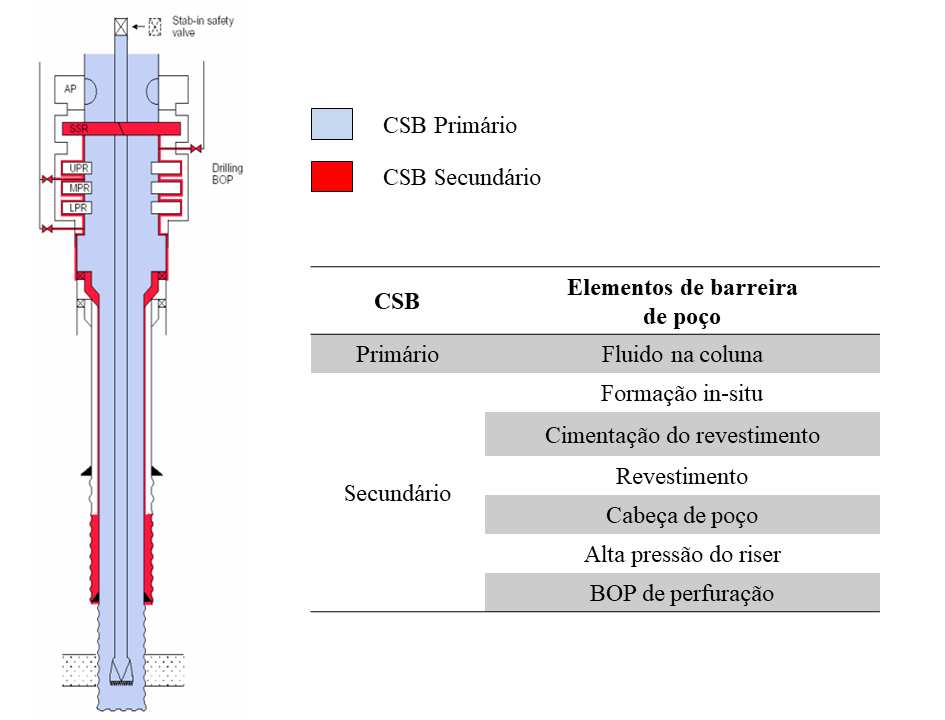
\includegraphics[scale=0.5]{Figures/CSB_corrigido.png}
%\vspace{12pt}
\caption{Elementos de barreira de poço em um processo de perfuração. Fonte: Adaptado de \citep{norge2013norsok}.}
\label{Fig2}
\end{center}
\end{figure}
%\vspace{8pt}

Na literatura são encontrados alguns trabalhos que envolvem a integridade em fluidos e revestimento. \cite{mendesanalise}, por exemplo, analisam diferentes critérios de assentamento de sapatas de revestimento e definem o peso de fluido de perfuração ótimo a partir da média entre as pressões de poros e de fratura.  \citep{melo2019integrated}, \citep{tenorio} e \citep{tenoriosoeaa}, por exemplo, avaliam a possibilidade de falha em revestimentos considerando os cenários de $kick$ de gás durante a perfuração, cimentação na instalação e uma análise integrada de $kick$ e cimentação, respectivamente. Para tanto, utiliza-se a ferramenta $Casing$ $Well$ (CWELL), a qual foi desenvolvida por \citep{costa} e está disponível no Sistema de Aplicações de Engenharia de Petróleo (SAEP).  

Neste contexto, o objetivo do trabalho é uma análise da integridade de elementos de barreira do CSB primário e secundário durante as fases de perfuração. Para tanto, é realizado o estudo de caso de um poço, analisando diferentes fluidos de perfuração e verificando a formação de $kick$ segundo o critério de janela operacional. Além disso, é avaliada a possibilidade de falha nos revestimentos por meio do $CWELL$, considerando os cenários de $kick$ de gás, poço completo de gás e perda de circulação total. 


% --------------------------------------------------------------------------
%\section{Revisão}\label{sec:revisão}%acho interessante não fazer essa seção, mas o conteúdo dela incluir na introdução
% --------------------------------------------------------------------------



% --------------------------------------------------------------------------
\section{Cenários de barreira de segurança} \label{sec:cenários}
% --------------------------------------------------------------------------

O poço foi idealizado por \citep{costa}.

\begin{figure}[!ht]
\begin{center}
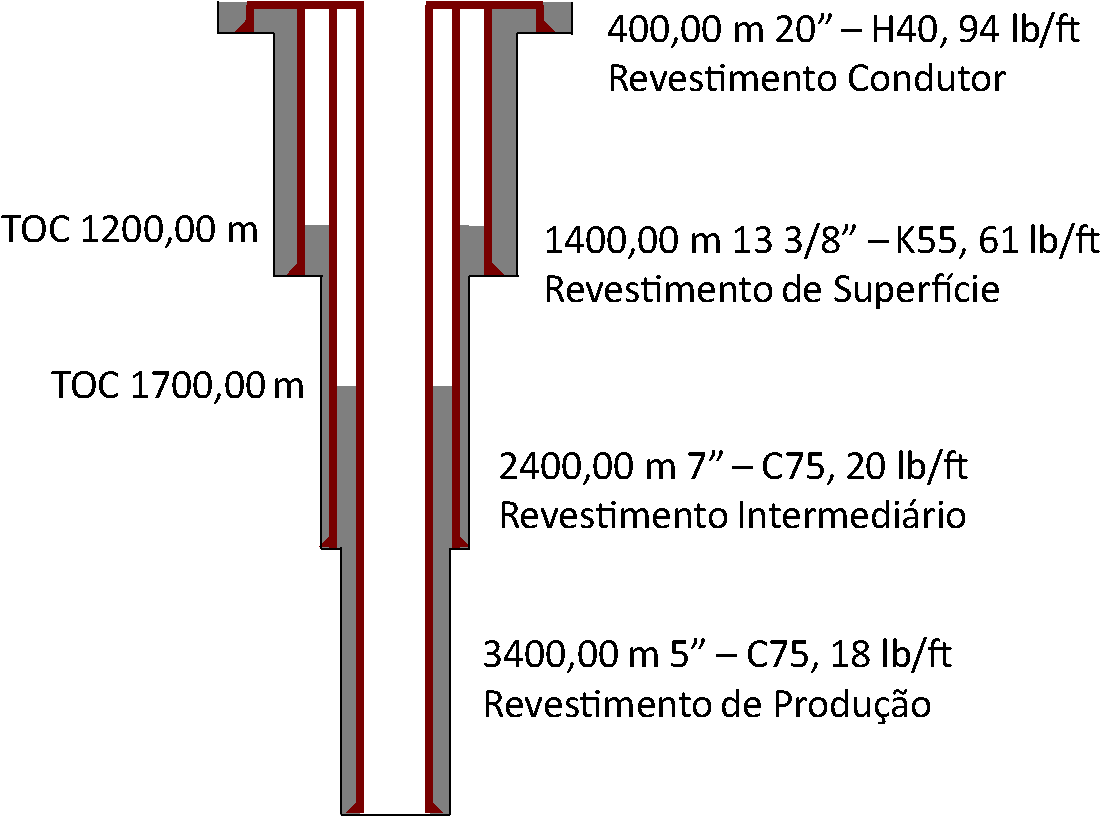
\includegraphics[scale=0.5]{Figures/poco.pdf}
%\vspace{12pt}
\caption{Esquema do modelo do poço.}
\label{poco}
\end{center}
\end{figure}



% Please add the following required packages to your document preamble:
% \usepackage{multirow}
\begin{table}[!ht]
\centering
\caption{Valores numéricos associados ao caso de estudo. Fonte: Adaptado de \citep{costa}}
\label{Table1}
\begin{tabular}{ccccccccc}
\multicolumn{1}{c|}{\multirow{2}{*}{Revestimento}} & \multicolumn{1}{c|}{\multirow{2}{*}{\begin{tabular}[c]{@{}c@{}}Diâmetro \\ Externo {[}pol{]}\end{tabular}}} & \multicolumn{3}{c|}{MD {[}m{]}} & \multicolumn{1}{c|}{\multirow{2}{*}{\begin{tabular}[c]{@{}c@{}}Hole Size \\ {[}m{]}\end{tabular}}} & \multicolumn{1}{c|}{\multirow{2}{*}{\begin{tabular}[c]{@{}c@{}}Densidade \\ da lama  {[}lb/gal{]}\end{tabular}}} & \multicolumn{1}{c|}{\multirow{2}{*}{Grade}} & \multirow{2}{*}{\begin{tabular}[c]{@{}c@{}}Peso \\ linear {[}lb/ft{]}\end{tabular}} \\ \cline{3-5}
\multicolumn{1}{c|}{} & \multicolumn{1}{c|}{} & Hanger & TOC & \multicolumn{1}{c|}{Base} & \multicolumn{1}{c|}{} & \multicolumn{1}{c|}{} & \multicolumn{1}{c|}{} &  \\ \hline
Condutor & 20 & 0 & 0 & 400 & 26 & 9.5 & H40 & 94 \\
Intermediário & 13 3/8 & 0 & 0 & 1400 & 17 1/2 & 10 & K55 & 61 \\
Produção & 7 & 0 & 1200 & 2400 & 8 1/2 & 12 & C75 & 32 \\ \hline
\end{tabular}
\end{table}

% --------------------------------------------------------------------------
\section{Resultados e discussão} \label{sec:resultados}
% --------------------------------------------------------------------------



% --------------------------------------------------------------------------
\section{Conclusão}\label{sec:Conclusão}
% --------------------------------------------------------------------------


\vspace{6pt}
\begin{center}
\begin{equation}
q_r = -4pr^2k\frac{dT}{dr}.
\label{Eq1}
\end{equation}
\end{center}
\vspace{6pt}



\vspace{8pt}
\begin{table}[!ht]
\centering
\caption{Coefficients in constitutive relations}
\label{Table1}
\vspace{0pt}
\begin{tabular}{ccc}
\hline
Constitutive relation & Nomenclature & Value \\[-2pt] \hline
Turbulent tensor & C$_{\mu}$ & 0.09 \\[-3pt]
Turbulent tensor & C$_{\mu b}$ & 0.69 \\[-3pt]
Lateral lift & C$_{L}$ & 0.08 \\[-3pt]
Virtual mass & C$_{VM}$ & 0.8 \\[-3pt] \hline
\end{tabular}
\end{table}
\vspace{8pt}


\begin{figure}[!ht]
\begin{center}
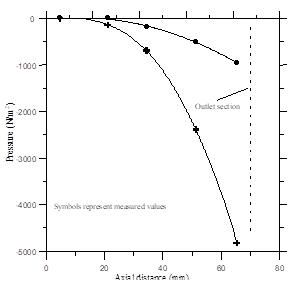
\includegraphics[scale=1.0]{Figures/Figure1.png}
\vspace{12pt}
\caption{Pressure variation along the nozzle: experimental data}
\label{Fig1}
\end{center}
\end{figure}
\vspace{8pt}


%-------------------------------------------------------------------------
\vspace{20pt}
\noindent \textbf{Acknowledgements.} This section should be positioned immediately after the Conclusion section. Type {Acknowledgements} in boldface, 10 pt Times New Roman type from left margin, leaving 20 pt line spacing before and 12pt after.
\vspace{12pt}

%--------------------------------------------------------------------------
\noindent \textbf{Authorship statement.} This section is mandatory and should be positioned immediately before the References section. The text should be exactly as follows:  The authors hereby confirm that they are the sole liable persons responsible for the authorship of this work, and that all material that has been herein included as part of the present paper is either the property (and authorship) of the authors, or has the permission of the owners to be included here. 

\bibliography{bibliography}

\end{document}
% --------------------------------------------------------------------------
